\documentclass[
 size=12pt,
 paper=smartboard, %a4paper, smartboard, screen
 mode=present, %present, handout, print
 display=slides, % slidesnotes, notes, slides
 style=tuliplab,  % TULIP Lab style
 pauseslide,
 fleqn,leqno,clock]{powerdot}

\usepackage{amssymb}
\usepackage{amsmath}
\usepackage{rotating}
\usepackage{graphicx}
\usepackage{boxedminipage}
\usepackage{media9}
\usepackage{rotate}
\usepackage{calc}
\usepackage[absolute]{textpos}
\usepackage{psfrag,overpic}
\usepackage{fouriernc}
\usepackage{pstricks,pst-node,pst-text,pst-3d,pst-grad}
\usepackage{moreverb,epsfig,color,subfigure}
\usepackage{color}
\usepackage{pstricks}
\usepackage{pstricks-add}
\usepackage{pst-text}
\usepackage{pst-node, pst-tree}
\usepackage{booktabs}
\usepackage{etex}
\usepackage{breqn}
\usepackage{multirow}
% \usepackage{pst-rel-points}

\usepackage{listings}
\lstset{frameround=fttt,
frame=trBL,
stringstyle=\ttfamily,
backgroundcolor=\color{yellow!20},
basicstyle=\footnotesize\ttfamily}
\lstnewenvironment{code}{
\lstset{frame=single,escapeinside=`',
backgroundcolor=\color{yellow!20},
basicstyle=\footnotesize\ttfamily}
}{}


\usepackage{hyperref}
\hypersetup{ % TODO: PDF meta Data
  pdftitle={Presentation Title},
  pdfauthor={Gang Li},
  pdfpagemode={FullScreen},
  pdfborder={0 0 0}
}


% \usepackage{auto-pst-pdf}
% package to show source code

\definecolor{LightGray}{rgb}{0.9,0.9,0.9}
\newlength{\pixel}\setlength\pixel{0.000714285714\slidewidth}
\setlength{\TPHorizModule}{\slidewidth}
\setlength{\TPVertModule}{\slideheight}
\newcommand\highlight[1]{\fbox{#1}}
\newcommand\icite[1]{{\footnotesize [#1]}}

\newcommand\twotonebox[2]{\fcolorbox{pdcolor2}{pdcolor2}{#1\vphantom{#2}}\fcolorbox{pdcolor2}{white}{#2\vphantom{#1}}}
\newcommand\twotoneboxo[2]{\fcolorbox{pdcolor2}{pdcolor2}{#1}\fcolorbox{pdcolor2}{white}{#2}}
\newcommand\vpspace[1]{\vphantom{\vspace{#1}}}
\newcommand\hpspace[1]{\hphantom{\hspace{#1}}}
\newcommand\COMMENT[1]{}

\newcommand\placepos[3]{\hbox to\z@{\kern#1
        \raisebox{-#2}[\z@][\z@]{#3}\hss}\ignorespaces}


%%%%%%%%%%%%%%%%%%%%%%%%%%%%%%%%%%%%%%%%%%%%%%%%%%%%%%%%%%%%%%%%%%%%%%%%%%
%%% title
%%% TODO: Customize to your Own Title, Name, Address
%%%
\title{FLIP(01) mid-term Presentation}
\author{Xiaojuan Cheng\\
Xi'an Shiyou University
% \href{mailto:gangli@acm.org}{gangli@acm.org}
% \and % more authors
}
%\date{11 November 2012}
\date{\today}


% Customize the setting of slides
\pdsetup{
% TODO: Customize the left footer, and right footer
rf={\copyright \emph{FLIP(01)}},
cf={FLIP(01) Presentation },
}


% Starts the document
\begin{document}

\maketitle

%%==========================================================================================
%%
\begin{slide}[toc=,bm=]{Outline}
  \tableofcontents[content=sections]
\end{slide}
%%
%%==========================================================================================

\section{Introduction}

\begin{slide}{Problem Description}
\begin{itemize}
\item<1->
This is a classification problem to predict seed varieties.
There are 210 samples, consistent of 7 features and 1 label.
The following is some requirements.
 \begin{itemize}
 \item<2->
    According to the given train data set,
    training a classified model and then using the model to predict the class of Wheat Seeds.
 \item<2->
    Estimated the error of the training classification model.\pause
\end{itemize}
\end{itemize}
\end{slide}

\section{Data Description}
%
\begin{slide}{Data Description}
\begin{itemize}
\item<1-> 
Attribute Information 
\item[1.]
There are 8 attributes, including 1 class attribute and 7 feature attributes. 
\item[2.]
The detailed description of the data is shown in the following table. 
\end{itemize}
\end{slide}

\begin{slide}{Data Description}

\begin{figure}
  \centering
  % Requires \usepackage{graphicx}
  \includegraphics[width=7in]{Figures/1.eps}\\
  \caption{Data}
  \label{Data}
\end{figure}

\end{slide}

\section{Features Distribution}

\begin{slide}{Features Distribution}
\begin{figure}
  \centering
  % Requires \usepackage{graphicx}
  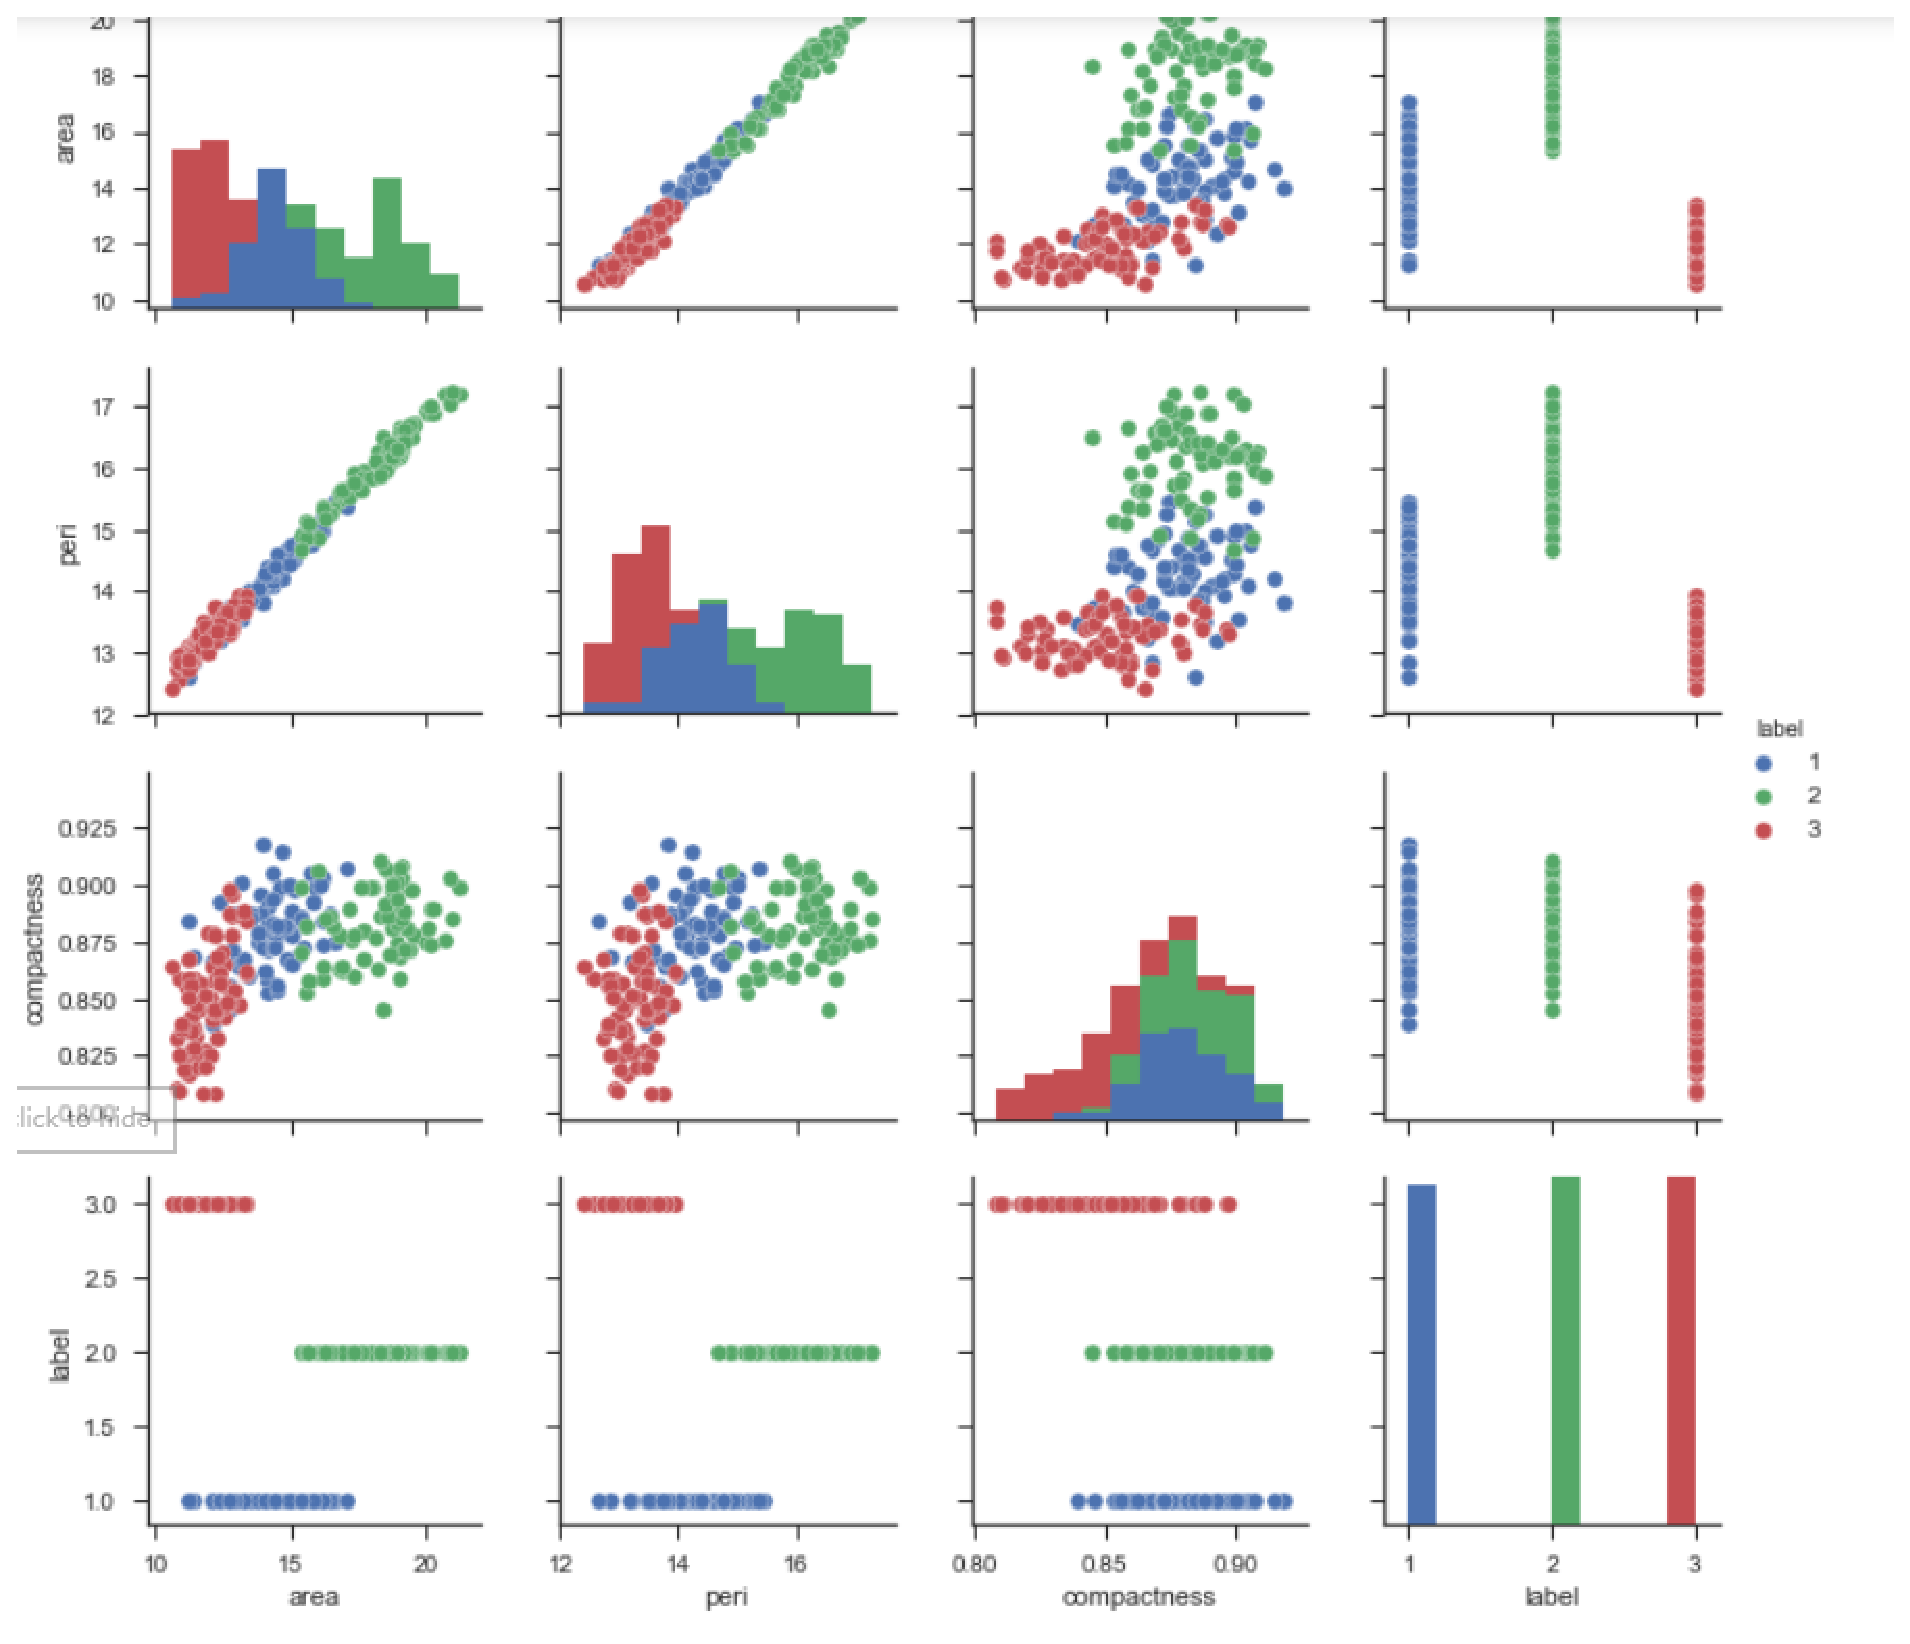
\includegraphics[width=5in]{Figures/2.eps}\\
  \caption{The distribution of features}
  \label{The distribution of features}
\end{figure}
\end{slide}

\section{Model Comparisions}

\begin{slide}{Model Comparisions}
\begin{figure}
  \centering
  % Requires \usepackage{graphicx}
  \includegraphics[width=6in]{Figures/3.eps}\\
  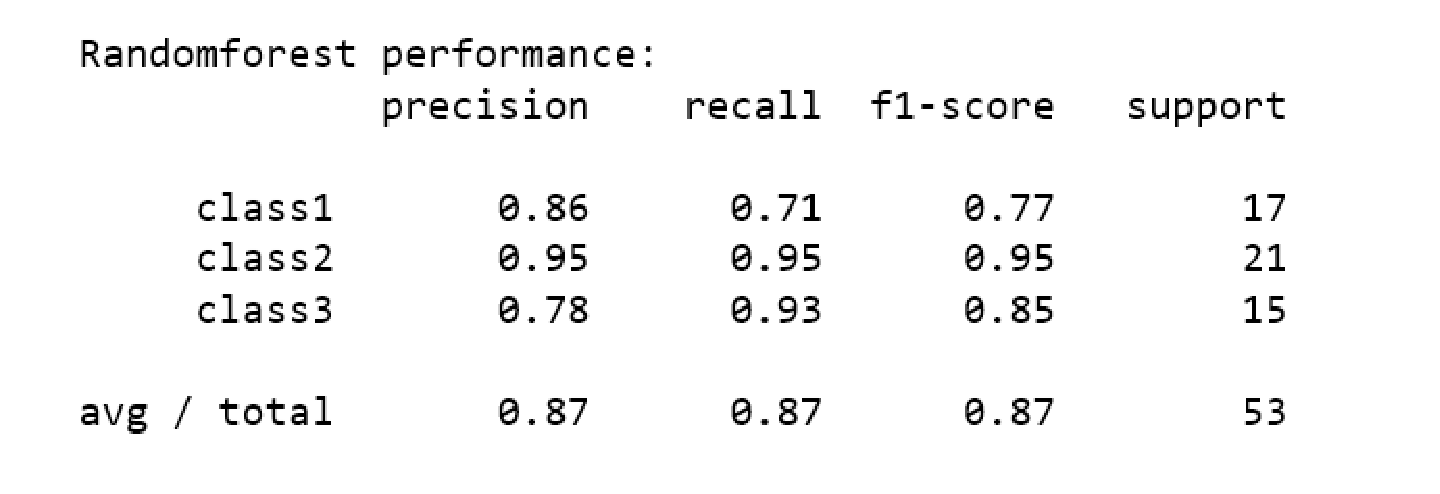
\includegraphics[width=6in]{Figures/4.eps}\\
  \caption{The Comparision of two models}
  \label{The Comparisions of two models}
\end{figure}

\end{slide}

\section{Conclusion}
\begin{slide}{Summary}
\begin{itemize}
\item From the above result presentation, we can find that
    \subitem KNN is better than Randomforest model.
    %\smallskip
%    \subitem PM2.5 is lowest in Guangzhou

\bigskip
\item From the feature distribution, we can find that
    \subitem Class1's data distribution is  more nearly Gaussian distribution.
    \smallskip
    \subitem The first two features are more interrelated.
%
%\bigskip
%\item
%The PM2.5 in Beijing is the worst in December and January
\end{itemize}
\end{slide}

\begin{wideslide}[toc=,bm=]{}
\centering
\vspace{\stretch{1}}
\twocolumn[
lcolwidth=0.35\linewidth,
rcolwidth=0.65\linewidth
]
{
% \centerline{\includegraphics[scale=.2]{tulip-logo.eps}}
}
{
\vspace{\stretch{1}}


\textcolor{black}{\scalebox{2.0}{Thank you \& Question}}


}
\vspace{\stretch{1}}
\end{wideslide}

\end{document}
\endinput
